\section{Tecnologías}

\subsection{Mongo}

MongoDB es una base de datos NoSQL (no solo SQL) orientada a documentos. Almacena
datos en una representación binaria llamada BSON (Binary JSON), la cual extiende
las capacidades de un objeto JSON (JavaScript Object Notation) para representar
tipos de datos como enteros, punto flotante, fechas, datos binarios, arreglos y sub-documentos o
documentos embebidos.

MongoDB posee un conjunto de  características que permiten la escalabilidad de una aplicación, entre ellas,
provee la habilidad e implementar la distribución geográfica de datos (sharding). Esto permite a la
base de datos ser escalada de forma horizontal con el uso de un conjunto de componentes de hardware o mediante
de la nube (cloud).

Adicionalmente, MongoDB esta diseñado para ser ejecutado en un sistema de múltiples nodos, por lo tanto,
en la presencia de un escalamiento horizontal, incluye la capacidad para la replicación
y sincronización de datos entre todos los componentes del sistema. De esta manera se garantiza la posibilidad
de implementar un servicio con alta disponibilidad \cite{10}.

\subsubsection{Replicación}

La replicación permite la redundancia de datos y el aumento de disponibilidad de los mismos en aplicaciones distribuidas.
Hace uso de múltiples servidores conectados entre sí y genera una replica de los datos en cada uno de ellos, de
esta manera se obtiene cierto nivel de tolerancia a fallos en caso de que un servidor de base de datos falle. 
También es posible mantener copias adicionales para propósitos específicos como recuperación en casos de desastre,
reportes o respaldos \cite{11}.

En MongoDB se hace uso de grupos de replica (replica sets) para almacenar las copias de datos en múltiples
servidores de base de datos. Un grupo de replica previene los tiempos de inactividad de la base de datos
en caso de errores y ayuda a escalar las operaciones de lectura. La recuperación de un miembro del grupo de
replica se realiza de forma automática. En un grupo de replica cualquier miembro puede actuar como nodo principal 
y el resto como secundario, por lo tanto, en caso de fallas de red o de hardware, un miembro del grupo
puede tomar el puesto de nodo primario después de haber sido elegido siguiendo un conjunto de reglas predefinidas.

Un grupo de replicas esta conformado por un nodo principal que realizara todas las operaciones de escritura, múltiples nodos 
secundarios y un nodo arbitro opcional, tal cual como lo muestra la siguiente figura:

\begin{figure}[H]
	\centering
		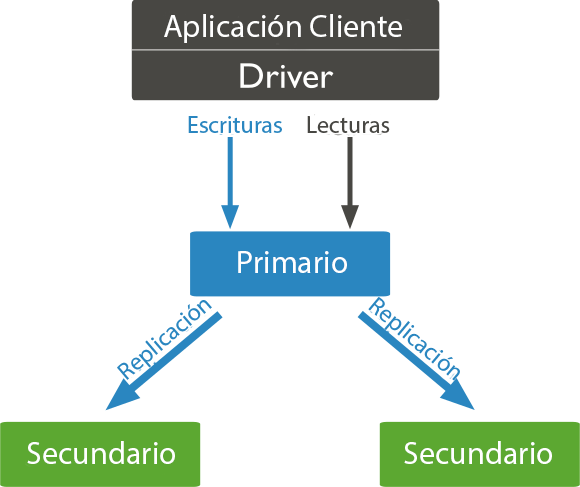
\includegraphics[width=.6\textwidth]{figures/replicas}
	\caption{Componentes de un grupo de replicas en MongoDB y su interacción con una aplicación cliente.}
	\label{fig:replicas}
\end{figure}

Para poder crear estos grupos es necesario tener un mínimo de tres nodos y escalar en números impares. Esto se 
debe a que cuando los componentes del grupo realicen la votación para elegir el nodo principal, se elimina la posibilidad de un
empate y el ganador es elegido de inmediato. 

En la siguiente figura se puede observar como los nodos del grupo se envían mensajes de diagnostico (heartbeats) para determinar
si sus vecinos son accesibles o no. En caso de que uno de estos heartbeat no obtenga una respuesta en 10 segundos, se marca dicho
destinarlo como inaccesibles.

\begin{figure}[H]
	\centering
		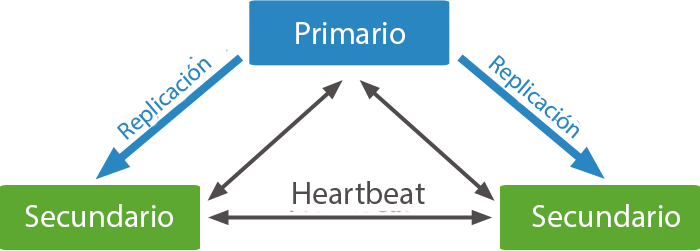
\includegraphics[width=.6\textwidth]{figures/heartbeat}
	\caption{Hearbeats en un grupo de replicación de MongoDB.}
	\label{fig:heartbeat}
\end{figure}


Los nodos secundarios se encargan de leer los datos presentes en el nodo primario y crear sus propia replica o copia del mismo.
Si, por alguna razón, el nodo primario deja de estar disponible, un nodo secundario elegible ejecutará una votación para 
elegir el siguiente nodo primario, tal como lo muestra la figura \ref{fig:failover}.
El primer nodo secundario en llevar a cabo la elección y recibir la mayoría de los botos se convierte en el nuevo nodo primario.


\begin{figure}[H]
	\centering
		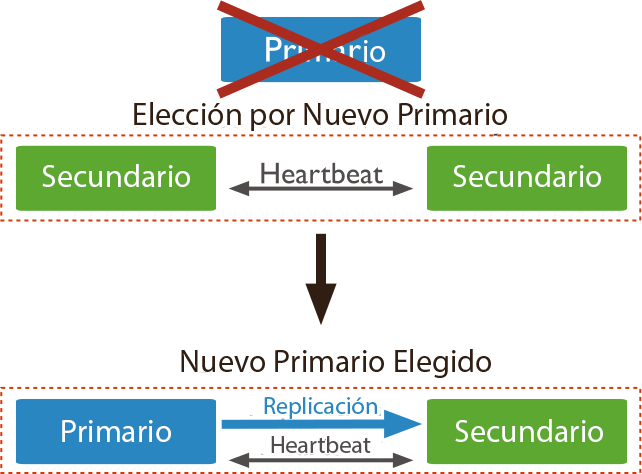
\includegraphics[width=.6\textwidth]{figures/failover}
	\caption{Proceso de elección de nuevo nodo primario en caso de errores.}
	\label{fig:failover}
\end{figure}


\subsubsection{Sharding}


\subsection{Celery}

\subsection{RabbitMQ}

\subsection{Flask}

\subsubsection{Flask AutoDoc}

% Is this subsection necessary?
\subsection{Wikipedia API}

